%Geometry.tex
\chapter{Geometry}\label{ch:geometry}
\begin{center}
{\small\em geometry descriptions...}
\end{center}

\section{Processing Models}
\begin{figure}[!h]
\centering
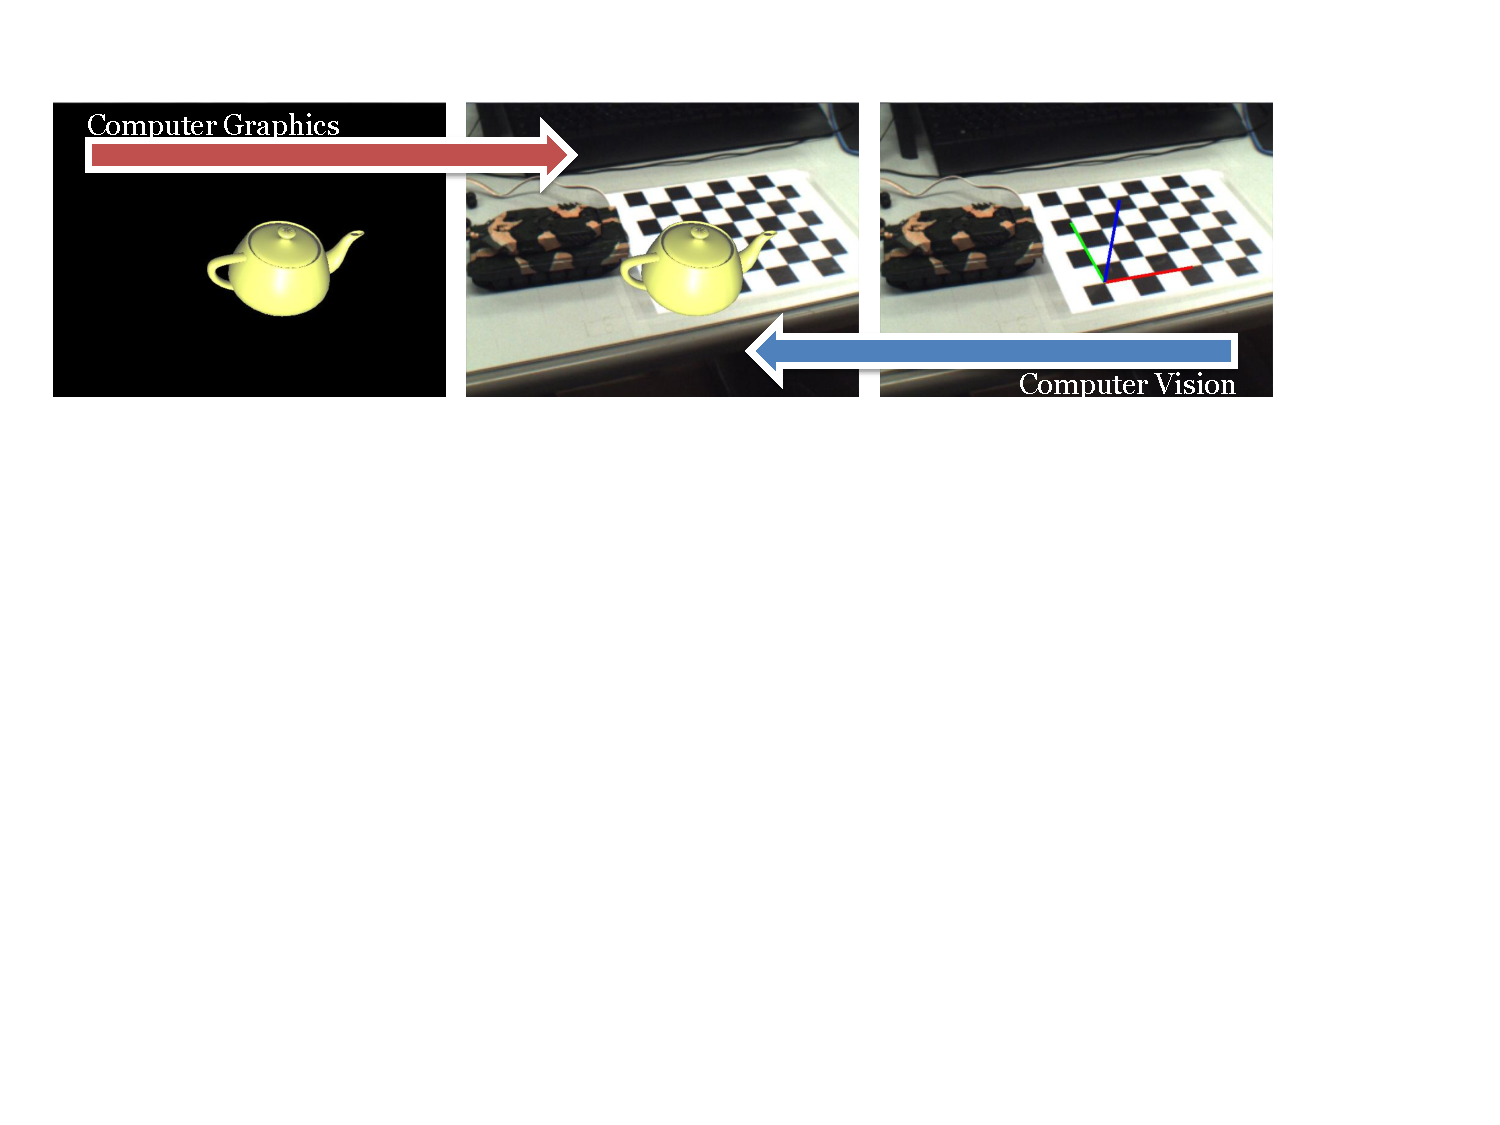
\includegraphics[width=6in]{images/processingmodel.pdf}
\caption{Processing Model using Computer Graphics and Computer Vision for Visual Computing}
\label{fig:processingmodel}
\end{figure}

\section{Camera Models}
A camera is a mapping between the 3D world (object space) and a 2D image\cite{CV_book_multiple_2000_Hartley}.

\begin{figure}[!h]
\centering
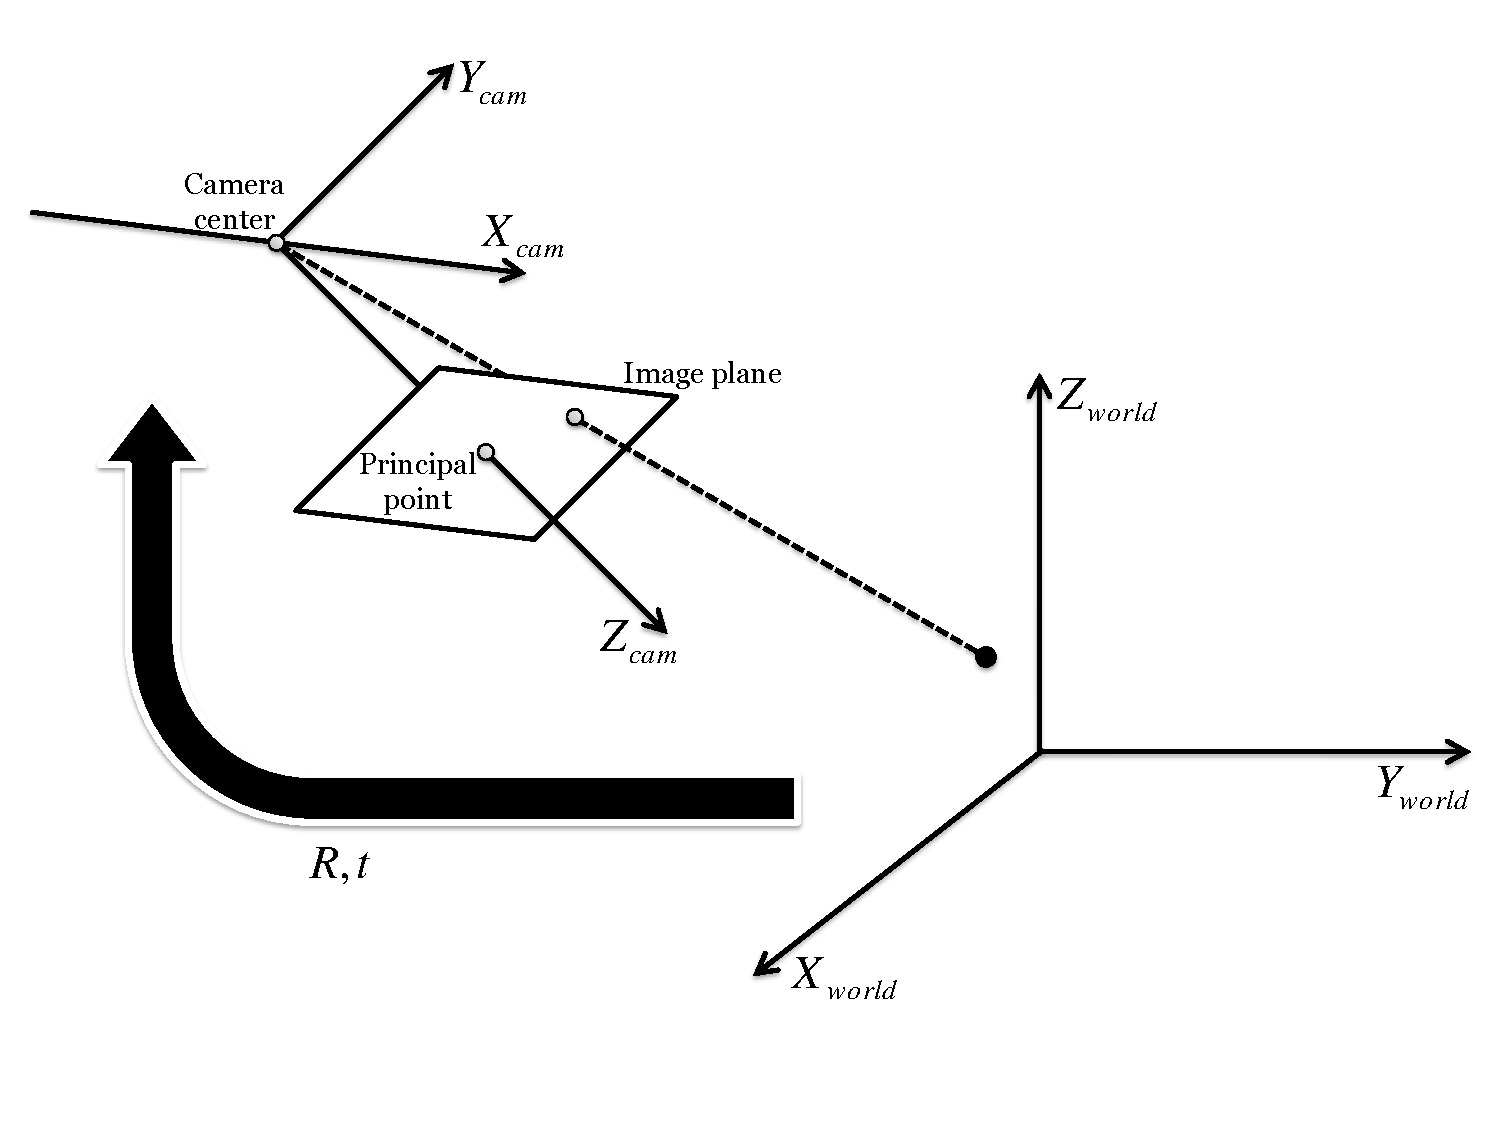
\includegraphics[width=6in]{images/cameramodel.pdf}
\caption{pinhole camera geometry}
\label{fig:cameramodel}
\end{figure}